% Presentación del Problem Set 3. La compila code/95_presentacion.R (paso del main); a mano, desde esta carpeta:
%   latexmk -pdf compare_equipo_4.tex
% Las figuras y las cifras del texto están en output/figures|tables/03_presentacion/ (las generan code/95-99).
\documentclass[aspectratio=169, 11pt]{beamer}
\usepackage[spanish, es-nodecimaldot]{babel}
\usepackage[T1]{fontenc}
\usepackage{fouriernc}   % New Century Schoolbook (texto y matemáticas)
\usepackage{graphicx}
\graphicspath{{../../output/figures/03_presentacion/}}
\newcommand{\tablas}{../../output/tables/03_presentacion}
\usepackage{booktabs}
\usepackage{array}
\usepackage{tikz}
\usetikzlibrary{positioning, arrows.meta}

% ---- Plantilla: Madrid (barra de título y pie de página de color) en verde oscuro ----
\usetheme{Madrid}
\usefonttheme{serif}     % Beamer usa sans por defecto; con esto el texto sale en Century
\setbeamertemplate{navigation symbols}{}
\definecolor{tinta}{HTML}{0B0B0B}
\definecolor{secundario}{HTML}{52514E}
\definecolor{verde}{HTML}{1E5631}
\definecolor{acento}{HTML}{1E5631}   % el mismo verde: diagrama y punto del ensamble en la figura
\definecolor{borde}{HTML}{898781}
\setbeamercolor{palette primary}{bg=verde, fg=white}
\setbeamercolor{palette secondary}{bg=verde!85!black, fg=white}
\setbeamercolor{palette tertiary}{bg=verde!70!black, fg=white}
\setbeamercolor{structure}{fg=verde}
\setbeamercolor{frametitle}{bg=verde, fg=white}
\setbeamercolor{title}{bg=verde, fg=white}
\setbeamercolor{normal text}{fg=tinta}
\setbeamerfont{frametitle}{series=\bfseries}
% Pie de página: autores | título | institución y número de diapositiva (la fecha solo va en la portada)
\setbeamertemplate{footline}{%
  \leavevmode%
  \hbox{%
    \begin{beamercolorbox}[wd=.333333\paperwidth, ht=2.25ex, dp=1ex, center]{author in head/foot}%
      \usebeamerfont{author in head/foot}\insertshortauthor
    \end{beamercolorbox}%
    \begin{beamercolorbox}[wd=.333333\paperwidth, ht=2.25ex, dp=1ex, center]{title in head/foot}%
      \usebeamerfont{title in head/foot}\insertshorttitle
    \end{beamercolorbox}%
    \begin{beamercolorbox}[wd=.333333\paperwidth, ht=2.25ex, dp=1ex, right]{date in head/foot}%
      \usebeamerfont{date in head/foot}\insertshortinstitute\hspace*{2em}%
      \insertframenumber{} / \inserttotalframenumber\hspace*{2ex}
    \end{beamercolorbox}}%
  \vskip0pt%
}

\input{\tablas/numeros.tex}
\input{\tablas/numeros_negocio.tex}   % moraleja 4: code/99_negocio.R

\title{Cuatro Moralejas sobre la Prediccion de Precios}
\author{Samuel Suárez, Maria Jose Pérez, Juan Manuel Lozano}
\institute[Uniandes]{Big Data y Machine Learning \\ Universidad de los Andes}
\date{Noviembre de 2026}

\begin{document}

\begin{frame}
  \titlepage
\end{frame}

% ---- 1. Modelo final ----
\begin{frame}{Modelo final: promedio ponderado de tres modelos}
  \centering
  \begin{tikzpicture}[
      caja/.style={draw=borde, rounded corners=3pt, align=center, minimum width=3.6cm, minimum height=1.25cm, font=\small},
      final/.style={draw=acento, line width=1pt, rounded corners=3pt, align=center, minimum width=4.6cm, minimum height=1.1cm, font=\small},
      flecha/.style={-{Stealth[length=2.2mm]}, draw=borde, line width=.7pt},
      peso/.style={font=\footnotesize\bfseries, fill=white, inner sep=1.5pt}]
    \node[caja] (nn)  at (-4.4, 0) {\textbf{NN STAR}\\ MAE \maeNN};
    \node[caja] (xgb) at (0, 0)    {\textbf{XGBoost}\\ MAE \maeXGB};
    \node[caja] (en)  at (4.4, 0)  {\textbf{ElasticNet}\\ MAE \maeEN};
    \node[final] (ens) at (0, -2.3) {\textbf{Promedio ponderado de precios}\\ MAE \maeEns};
    \draw[flecha] (nn.south)  -- node[peso] {\pesoNN\,\%}  (ens.north west);
    \draw[flecha] (xgb.south) -- node[peso] {\pesoXGB\,\%} (ens.north);
    \draw[flecha] (en.south)  -- node[peso] {\pesoEN\,\%}  (ens.north east);
  \end{tikzpicture}

  \vspace{1.2em}
  \raggedright\small
  \begin{itemize}
    \item \textbf{NN STAR:} red neuronal con tres ramas que se suman: estructura del inmueble, ubicación y texto del anuncio.
    \item \textbf{XGBoost:} árboles con todas las variables y el precio por m$^2$ de los 5 y 20 anuncios más cercanos.
    \item \textbf{ElasticNet:} regresión lineal penalizada con un resumen de la descripción.
  \end{itemize}

  \vfill
  {\scriptsize\color{secundario} MAE público en Kaggle, en millones de pesos.}
\end{frame}

% ---- 2. Por qué funciona ----
\begin{frame}{Por qué la combinación tiene menor error que cada modelo}
  \begin{columns}[T]
    \begin{column}{.44\textwidth}
      \small
      \begin{itemize}
        \item La red aprende la ubicación de las coordenadas y del texto; el XGBoost, del precio de los vecinos.
        \item Por eso se equivocan en anuncios distintos: la correlación estimada de sus errores es \corrErrores.
        \item Al promediar, parte de esos errores se cancela.
        \item Pesos: \pesoNN\,\% red, \pesoXGB\,\% XGBoost y \pesoEN\,\% ElasticNet.
      \end{itemize}
    \end{column}
    \begin{column}{.54\textwidth}
      \centering
      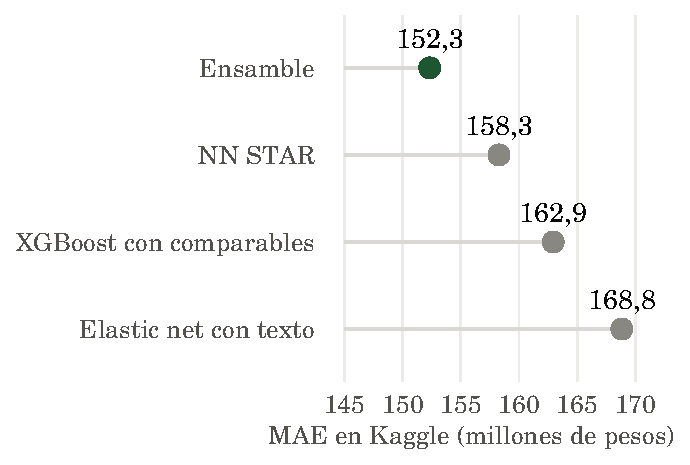
\includegraphics[width=\linewidth]{mae_ensamble.pdf}
    \end{column}
  \end{columns}

  \vfill
  
\end{frame}

% ---- Datos: qué datos prioriza cada modelo (SHAP) ----
\begin{frame}{Datos}
  \begin{columns}[T]
    \begin{column}{.62\textwidth}
      \centering
      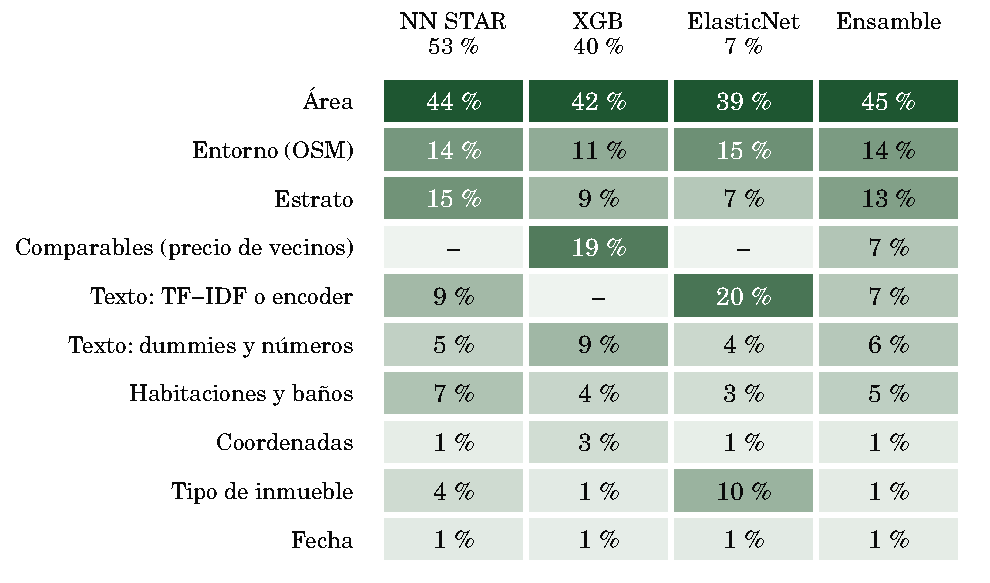
\includegraphics[width=\linewidth, height=.72\textheight, keepaspectratio]{shap_grupos.pdf}
    \end{column}
    \begin{column}{.36\textwidth}
      \small
      \vspace{1.2em}
      \begin{itemize}\setlength{\itemsep}{8pt}
        \item El área domina en todos los modelos.
        \item Cada modelo saca el nivel de la ubicación de una fuente distinta: la red del estrato y el entorno, el XGB del precio de los vecinos.
        \item El ElasticNet se apoya más en el encoder de texto.
      \end{itemize}
    \end{column}
  \end{columns}

  \vfill
  {\scriptsize\color{secundario} Participación de cada grupo de datos en la importancia total de cada modelo: promedio del valor absoluto de los SHAP (Lundberg y Lee, 2017) en 2.000 anuncios del test.}
\end{frame}

% ---- Moraleja 1 (interpretabilidad), diapositiva A: el problema y el STAR ----
\begin{frame}{Moraleja 1: Un modelo interpretable casi iguala al ensamble}
  \small
  \begin{itemize}\setlength{\itemsep}{9pt}
    \item El ensamble del equipo es difícil de interpretar: su XGBoost cruza todas las variables, así que el efecto de la ubicación cambia con el área, el texto y todo lo demás.
    \item Un STAR (Mayer et al., 2022) suma una función por grupo de variables:
      \[ \log \text{precio} = f_{\text{estructura}} + f_{\text{ubicación}} + f_{\text{texto}} \]
      Cada función solo ve su grupo. El efecto de un grupo es el mismo para todos los anuncios y se lee directamente.
    \item Frente a explicar una caja negra con valores de Shapley:
    \begin{itemize}\footnotesize\setlength{\itemsep}{3pt}
      \item Es exacto: la componente de cada grupo es su valor de Shapley; no hay que aproximar.
      \item Es global: un solo efecto por grupo, no uno por anuncio que depende del resto de variables.
      \item Cada componente se puede usar por fuera del modelo: el encoder de texto del ElasticNet sale de un XGB STAR.
    \end{itemize}
  \end{itemize}
\end{frame}

% ---- Moraleja 1, diapositiva B: estructura de la combinación STAR final (m48) ----
\begin{frame}{Moraleja 1: Un modelo interpretable casi iguala al ensamble}
  \centering
  \begin{tikzpicture}[
      grupo/.style={draw=verde, line width=.8pt, rounded corners=3pt, align=left, text width=3.3cm, minimum height=.95cm, font=\scriptsize},
      celda/.style={draw=borde, rounded corners=3pt, align=center, text width=3.4cm, minimum height=.95cm, font=\scriptsize},
      suma/.style={draw=verde, line width=.8pt, rounded corners=3pt, align=center, text width=3.2cm, minimum height=.95cm, font=\scriptsize},
      flecha/.style={-{Stealth[length=1.8mm]}, draw=borde, line width=.6pt},
      cab/.style={font=\footnotesize\bfseries}]
    \node[cab] at (-4.6, 1.25) {Grupo de variables};
    \node[cab] at (-0.6, 1.25) {NN STAR (60\,\%)};
    \node[cab] at ( 3.3, 1.25) {XGB STAR (40\,\%)};
    \node[cab] at ( 7.1, 1.25) {Componente final};
    \foreach \y/\g/\nn/\xg/\f in {
        0/{\textbf{Estructura}\\área, baños, habitaciones, tipo, dummies del texto}/{una capa lineal:\\un coeficiente por variable}/{árboles de una sola variable}/{$0{,}6 f^{NN}_{\text{est}} + 0{,}4 f^{XGB}_{\text{est}}$},
        -1.2/{\textbf{Ubicación}\\coordenadas, distancias, estrato, valor catastral}/{rama profunda 64-32-16\\+ atajo lineal}/{árboles solo con ubicación\\(+ precio de los vecinos)}/{$0{,}6 f^{NN}_{\text{ubi}} + 0{,}4 f^{XGB}_{\text{ubi}}$},
        -2.4/{\textbf{Texto}\\1.000 términos TF-IDF}/{rama profunda 64-32-16\\+ atajo lineal}/{árboles solo con términos}/{$0{,}6 f^{NN}_{\text{txt}} + 0{,}4 f^{XGB}_{\text{txt}}$}} {
      \node[grupo] (g\y) at (-4.6, \y) {\g};
      \node[celda] (n\y) at (-0.6, \y) {\nn};
      \node[celda] (x\y) at ( 3.3, \y) {\xg};
      \node[suma]  (s\y) at ( 7.1, \y) {\f};

    }
  \end{tikzpicture}

  \vspace{.4em}
  \raggedright\small
  \begin{itemize}\setlength{\itemsep}{3pt}
    \item $\log \text{precio} = \sum_g f_g$. Ningún grupo se cruza con otro, ni en la red ni en los árboles. El promedio de dos STAR sigue siendo un STAR.
    \item MAE en Kaggle: \kStar{} (la red sola, \kNNstar; el ensamble del equipo, \maeEns).
  \end{itemize}
\end{frame}

% ---- Moraleja 1, diapositiva C: mapas de la componente de ubicación ----
\begin{frame}{Moraleja 1: Un modelo interpretable casi iguala al ensamble}
  \begin{columns}[T]
    \begin{column}{.64\textwidth}
      \centering
      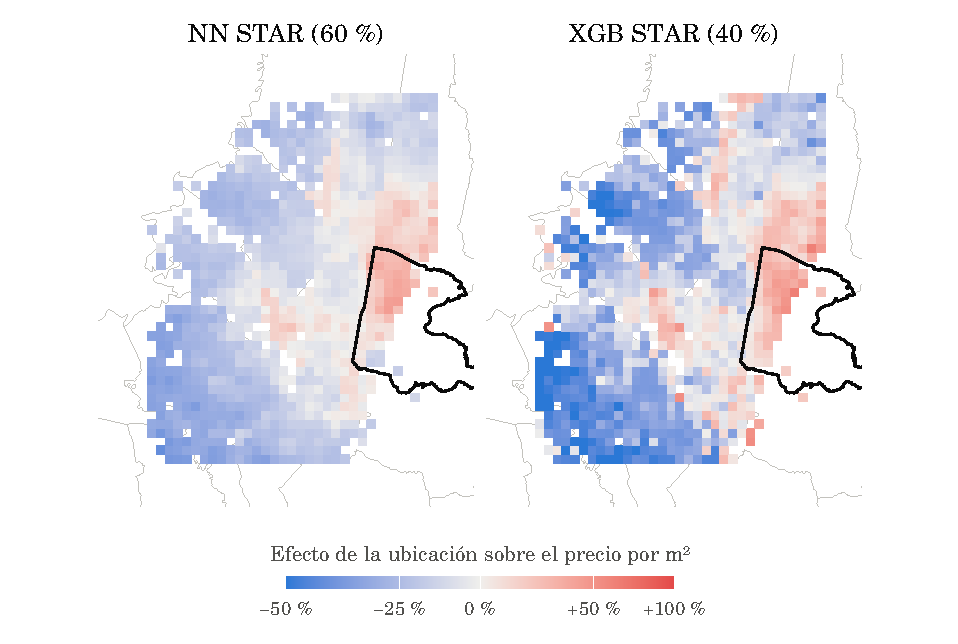
\includegraphics[width=\linewidth, height=.78\textheight, keepaspectratio]{mapas_ubicacion.pdf}
    \end{column}
    \begin{column}{.34\textwidth}
      \small
      \vspace{1.5em}
      \begin{itemize}\setlength{\itemsep}{8pt}
        \item Cada mapa es la componente de ubicación de un modelo: cuánto cambia el precio por m$^2$ solo por dónde está el inmueble.
        \item Los dos modelos ven la misma ciudad ($r = \corUbicacion$).
        \item La red da un mapa suave; el XGB, con el precio de los vecinos, uno más detallado.
      \end{itemize}
    \end{column}
  \end{columns}

  \vfill
  {\scriptsize\color{secundario} Mediana de la componente de ubicación en celdas de 500 m, train y test. Contorno negro: Chapinero.}
\end{frame}

% ---- 4. Moraleja 1A: el encoder y las dummies ----
\begin{frame}{Moraleja 2: Representar bien el texto importa...}
  \begin{columns}[T]
    \begin{column}{.52\textwidth}
      \centering
      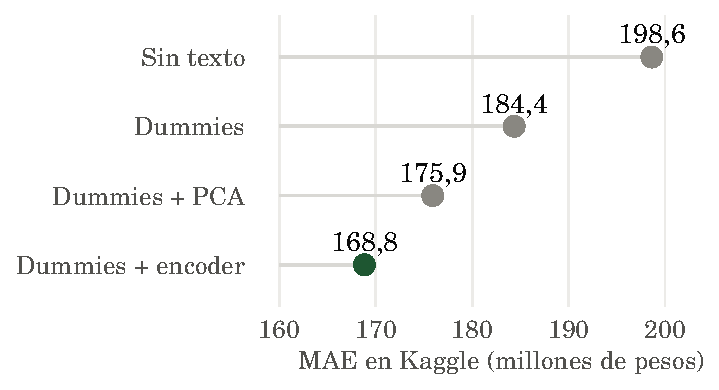
\includegraphics[width=\linewidth, height=.55\textheight, keepaspectratio]{texto_kaggle_en.pdf}\\[-.3em]
      {\scriptsize\color{secundario} ElasticNet con las mismas variables base}
    \end{column}
    \begin{column}{.45\textwidth}
      \small
      \vspace{1.5em}
      \begin{itemize}\setlength{\itemsep}{10pt}
        \item Veamos en el caso del EN (es igual para los otros modelos)
        \item El encoder de este modelo es un valor dado a cada anuncio por XGB STAR
        \item El encoder se entrena con el precio y mejora \encVsPca{} M frente al PCA.
        \item Las dummies recuperan números que el TF-IDF pierde (piso, antigüedad, parqueaderos).
      \end{itemize}
    \end{column}
  \end{columns}
\end{frame}

% ---- 5. Moraleja 1B: por qué el PCA rinde menos ----
\begin{frame}{Moraleja 2: Representar bien el texto importa...}
  \small
  El PCA busca varianza, no precio, y su primera componente son plantillas de inmobiliarias.

  \vspace{1em}
  \begin{center}
    \footnotesize\input{\tablas/pca_ejemplo.tex}
  \end{center}
\end{frame}

% ---- 6. Moraleja 1C: cómo leen el texto la red y los árboles ----
\begin{frame}{Moraleja 2: ...pero el modelo que usa el texto no importa tanto}
  \begin{columns}[T]
    \begin{column}{.46\textwidth}
      \centering
      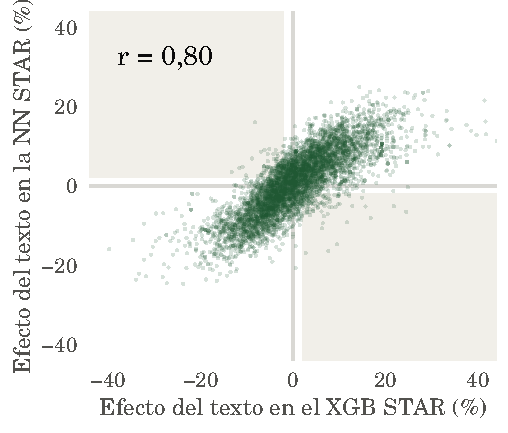
\includegraphics[width=\linewidth, height=.62\textheight, keepaspectratio]{texto_dispersion.pdf}
    \end{column}
    \begin{column}{.52\textwidth}
      \footnotesize
      \begin{itemize}\setlength{\itemsep}{5pt}
        \item El efecto del texto en la NN STAR es muy cercano al efecto del texto en el XGB STAR ($r = \corTextoModelos$).
        \item Aun así, hay palabras en que difieren.
        \begin{itemize}\scriptsize
          \item Los anuncios con nombre de inmobiliaria (PADS, Rentahouse) tienen más peso del texto en la NN STAR.
          \item Los anuncios con amenidades de lujo (ascensor privado, para estrenar) tienen más peso del texto en el XGB STAR.
          \item Los árboles se quedan con pocas palabras de efecto fuerte (amenidades); la red reparte el peso entre muchas, incluidas las plantillas de cada inmobiliaria.
        \end{itemize}
    
      \end{itemize}
    \end{column}
  \end{columns}

  \vfill
\end{frame}

% ---- Moraleja 3 (validación), diapositiva A: correlación entre la validación y Kaggle ----
\begin{frame}{Moraleja 3: Mejorar la validación no siempre mejora en Kaggle}
  \centering
  {\small Correlación de Pearson entre cada medida de validación y el MAE en Kaggle}\\[.8em]
  \footnotesize\input{\tablas/validacion_kaggle.tex}

  \vspace{.8em}
  {\footnotesize TWCV: la CV pondera cada anuncio para que el train se parezca al test (Brenning y Suesse, 2026).}

  \vfill
  \raggedright
  {\scriptsize\color{secundario} \nModTabla{} modelos subidos a Kaggle. Se excluyen los que usan el precio de los vecinos o la CV por edificio, cuya validación no es comparable, y las combinaciones.}
\end{frame}

% ---- Moraleja 3, diapositiva B: consecuencias ----
\begin{frame}{Moraleja 3: Mejorar la validación no siempre mejora en Kaggle}
  \small
  \begin{itemize}\setlength{\itemsep}{10pt}
    \item Cada familia de modelos sirve mejor con una validación distinta. El ElasticNet con el TWCV, las redes con el promedio por localidad.
    \item Con el precio de los vecinos, la CV deja de servir: el XGB con comparables marca \cvXGBcomp{} M en la CV y \kXGBcomp{} M en Kaggle.
    \item Como consecuencia, las redes afinadas fueron peores: mejor TWCV (\twAfinada{} frente a \twBase), peor Kaggle (\kAfinada{} frente a \kBase). Lo mismo con la primera red (\kAfinadaUno{} frente a \kBaseUno).
    \item ¿Entonces cuál fue la medida más consistente de mejora?
  \end{itemize}
  \pause
  \vspace{.6em}
  \begin{center}
    \textbf{El valor medio de las predicciones}\\[.3em]
    {\footnotesize $r = \corMediaTodos$ con el MAE en Kaggle en los \nModKaggle{} modelos.}
  \end{center}
\end{frame}

% ---- Moraleja 4 (negocio), diapositiva A: los modelos subpredicen lo caro (code/99_negocio.R) ----
\begin{frame}{Moraleja 4: Donde está la plata, el modelo se equivoca más}
  \begin{columns}[T]
    \begin{column}{.52\textwidth}
      \centering
      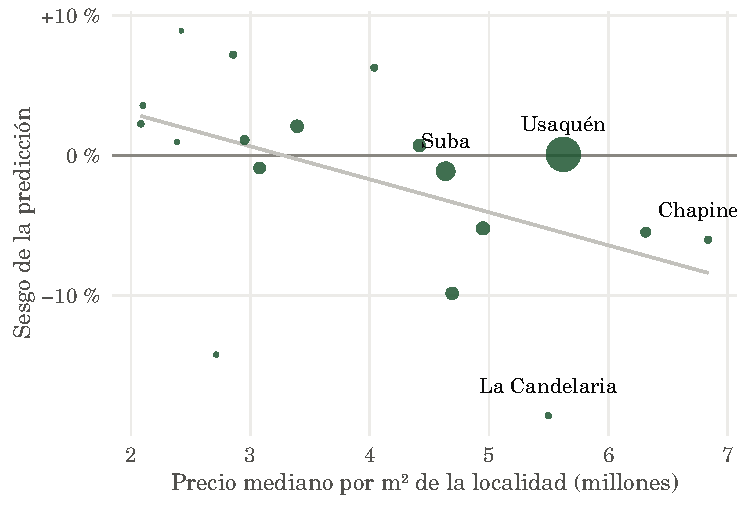
\includegraphics[width=\linewidth, height=.68\textheight, keepaspectratio]{sesgo_localidades.pdf}
    \end{column}
    \begin{column}{.46\textwidth}
      \small
      \vspace{.8em}
      \begin{itemize}\setlength{\itemsep}{8pt}
        \item Si subir las predicciones casi siempre mejora el modelo, el modelo está subprediciendo.
        \item En la validación, los tres modelos subpredicen Chapinero (\sesgoChapRed, \sesgoChapXGB{} y \sesgoChapEN\,\%). Multiplicar por \kChapMin{}--\kChapMax{} baja el MAE.
        \item Entre más cara la localidad, más se subpredice ($r$ entre $\corLocEN$ y $\corLocXGB$).
      \end{itemize}
    \end{column}
  \end{columns}

  \vfill
  {\scriptsize\color{secundario} Predicciones fuera de muestra de la CV por localidad: cada localidad se predice sin haberla visto. Figura: NN STAR; tamaño del punto: número de anuncios.}
\end{frame}

% ---- Moraleja 4, diapositiva B: los inmuebles excepcionales ----
\begin{frame}{Moraleja 4: Donde está la plata, el modelo se equivoca más}
  \begin{quote}\itshape
    ``That is simply because if Messi is an outlier, and since he is an outlier, you can never approximate him.''\\
    \upshape\hfill\footnotesize Cunningham (2021), sobre el control sintético
  \end{quote}

  \vspace{.4em}
  \small
  \begin{itemize}\setlength{\itemsep}{8pt}
    \item El \pctMessi\,\% de los anuncios de Chapinero cuesta más por m$^2$ que el 95\,\% del resto de la ciudad (\pNoventaCinco{} M por m$^2$).
    \item En esos anuncios la red subpredice \sesgoMessiRed\,\%. En el resto de Chapinero, \sesgoRestoRed\,\%.
    \item A diferencia de SCM, nuestors modelos extrapolan, pero mal. La red con sus atajos lineales (\sesgoMessiRed\,\%), los árboles no pasan del valor de sus hojas (\sesgoMessiXGB\,\%).
  \end{itemize}
\end{frame}

% ---- Moraleja 4, diapositiva C: ¿se puede ganar plata? ----
\begin{frame}{Moraleja 4: Donde está la plata, el modelo se equivoca más}
  \small
  \begin{itemize}\setlength{\itemsep}{10pt}
    \item En contra: en Chapinero (usando datos de test) el error mediano es \mapeChap\,\% y solo el \dentroDiezChap\,\% de los anuncios queda a menos de 10\,\%. Un inmueble de lujo quedaría valorado \sesgoMessiRed\,\% por debajo.
    \item A favor: sin los inmuebles excepcionales, el sesgo casi desaparece (\sesgoRestoRed\,\%). Sirve como primera valoración.
    \item Alternativa: un barrio cercano a la media de la ciudad. En Usaquén y Suba el sesgo es de \sesgoUsaquen{} y \sesgoSuba\,\%, aunque el error relativo sigue cerca de \mapeUsaquen\,\%.
  \end{itemize}
\end{frame}

\end{document}
